\section{Measurement And Data Analysis}

	\subsection{Presentation Of Data}
		\begin{table}[htbp]
			\centering
			\begin{tabular}{|c|c|c|c|c|c|c|}
				\hline
				\multicolumn{2}{|c|}{} &\multicolumn{5}{|c|}{Aperture: 4mm} \\
				\cline{3-7}
				\multicolumn{2}{|c|}{}  & $\lambda = 365nm$ & $\lambda = 405nm$ & $\lambda = 435nm$ & $\lambda = 546nm$ & $\lambda = 577nm$\\\hline
				
				\multirow{10}{*}{\rotatebox{90}{Data}}  & -2V & \(-3.4A\) &  \(-12A \)&  \(-11.1A\) &  \(-9.3A\) &  \(-3.7A\) \\\cline{2-7}    
				&-1.5V & \(209A\) &  \(3.2A\) &  \(-6.5A\) &  \(-9A\) &  \(-3.6A\) \\\cline{2-7}
				&-1.0V & \(637A\) &  \(101A\) &  \(104.7A\) &  \(-8.3A\) &  \(-3.5A\) \\\cline{2-7}
				& -0.5V & \(1084A\) &  \(236A\) &  \(316A\) &  \(98.3A\) &  \(22A\) \\\cline{2-7}
				& 0V & \(1600A\)&   \(385A\)&   \(540A\)    & \(350A\) &    \(125.2A\) \\ \cline{2-7}
				& 5V& \(8570A\) & \(2160A\)& \(3060A\)&   \(2040A\)&   \(721A\)\\\cline{2-7}
				& 10V& \(14600A\) & \(3660A\)& \(5180A\)&   \(3170A\)&   \(1141A\)\\
				\cline{2-7}
				& 15V& \(19670A\) & \(4860A\)& \(6800A\)&   \(4000A\)&   \(1401A\)\\\cline{2-7}
				& 20V& \(23700A\) & \(5900A\)& \(8250A\)&   \(4610A\)&   \(1577A\)\\\cline{2-7}
				& 25V& \(27300A\) & \(5900A\)& \(8250A\)&   \(4610A\)&   \(1577A\)\\\cline{2-7}
				& 30V& \(30200A\) & \(7480A\)& \(10400A\)&   \(5290A\)&   \(1790A\)\\
				\hline  
				
			\end{tabular}
			\caption{Experimental Data}
			\label{tbl:data}
		\end{table}
	
		\begin{figure}[H]
			\centering
			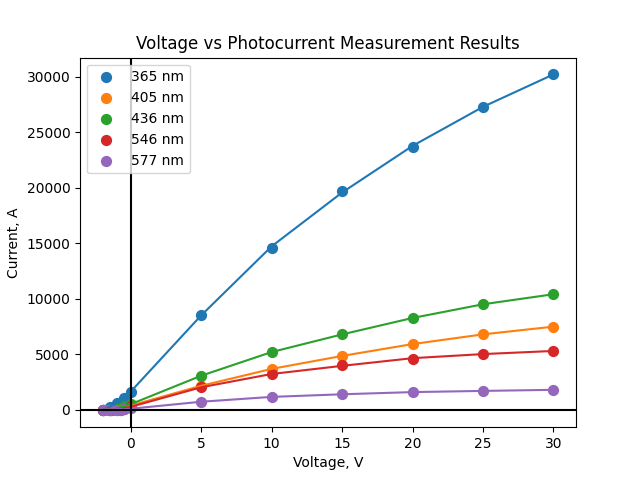
\includegraphics[width=10cm]{images/plot1a_pe.png}
			\caption{Voltage versus current plot of the data in Table \ref{tbl:data}.}
			\label{fig:pl1a}
		\end{figure}
	
		\begin{figure}[H]
			\centering
			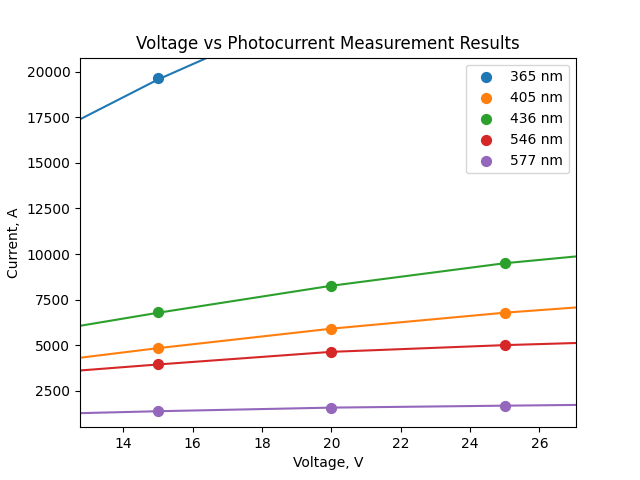
\includegraphics[width=10cm]{images/plot1b_pe.png}
			\caption{Voltage versus current plot of the data in Table \ref{tbl:data}, enlarged to highlight the difference in current.}
			\label{fig:pl1b}
		\end{figure}
	
		\begin{table}[htbp]
			\centering
			\begin{tabular}{ |l|l|l| }
				\hline
				\multicolumn{2}{ |c| }{Stopping Voltages, V: Current = 0A} \\
				\hline
				365 nm & -1.944 V\\ \hline
				405 nm& -1.55 V\\ \hline
				436 nm& -1.331 V\\ \hline
				546 nm& -0.784 V\\ \hline
				577 nm& -0.683 V\\ \hline
				
			\end{tabular}
			\caption{Stopping Voltage Data}
			\label{tbl:stpv}
		\end{table}
		
	
		\begin{figure}[H]
			\centering
			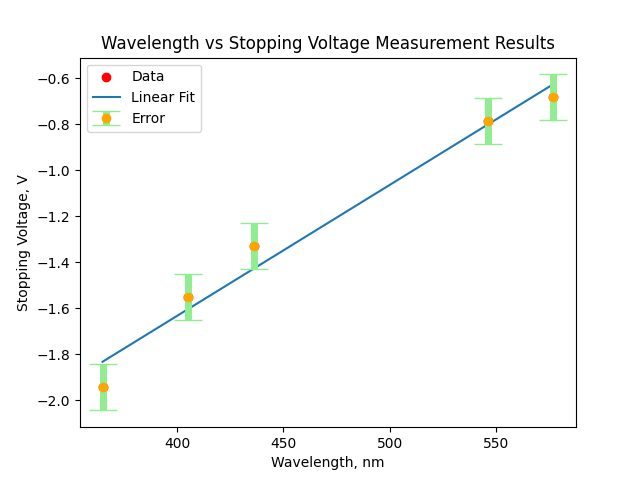
\includegraphics[width=10cm]{images/plot2_pe.png}
			\caption{Voltage versus current plot of the data in Table \ref{tbl:stpv}.}
			\label{fig:plt2}
		\end{figure}
	